\documentclass{article}
\usepackage{amsmath}
\usepackage{pdfpages}
\usepackage{xeCJK}
\usepackage{hyperref}
\usepackage{listings}
\lstset{
 columns=fixed,       
 numbers=left,                                        % 在左侧显示行号
 numberstyle=\tiny\color{gray},                       % 设定行号格式
 frame=single,                                          % 不显示背景边框
 keywordstyle=\color[RGB]{40,40,255},                 % 设定关键字颜色
 numberstyle=\footnotesize\color{darkgray},           
 commentstyle=\it\color[RGB]{0,96,96},                % 设置代码注释的格式
 stringstyle=\rmfamily\slshape\color[RGB]{128,0,0},   % 设置字符串格式
 showstringspaces=false,                              % 不显示字符串中的空格
 language=c++,                                        % 设置语言
}
\newcommand{\paper}[2]{\hyperlink{./papers/#1.pdf.#2}{(P#2)}}
\newcommand{\book}[2]{\href[page=#2]{./books/#1.pdf}{(P#2)}}


\title{Evolutionary Computing and Machine Learning}
\author{陈辉}
\date{}
\begin{document}
\maketitle
\tableofcontents
\newpage
\part{文献}
\section{\textit{Population-Based-Training-of-Neural-Networks}}
\paper{Population-Based-Training-of-Neural-Networks}{1}
\subsection{Introduction}
\paragraph{Keypoints of The Problem}

\begin{itemize}
		\item Hyperparameters tuning is essential.
		\href{https://en.wikipedia.org/wiki/Hyperparameter\_optimization}{Wiki}.
		\item Non-stationary problems might lead to non-stationary hyperparameters.
		\item Tow main tuning tracks:
\begin{itemize}
		\item Parallel search. 
		\item Sequential search.
\end{itemize}
\end{itemize}

\paragraph{Brief Introduction to PBT}
\paragraph{What PBT can do}

\subsection{Related Work}
\paragraph{Bayesian optimisation framework}
\paragraph{Main thoughts of PBT for training}A misture way: Parameters are more likely to be trained(partially) in standard way, while the hyperparameters are evolved(relatively slowly).

\subsection{Population Based Training}
\paragraph{Main idea}
\begin{itemize}
\item Training with a population that each member has different parameters and hyper parameters.
\item In each iteration, a member takes steps and offer its weights, hyperparameters and evaluation. This is the main \textbf{communication} among members.
\item Each member \textbf{\textit{exploit}} the best weights and hyperparameters among the whole polulation, then \textbf{\textit{explore}} new branches for next step.
\end{itemize}
\textbf{Remark. }Can we treat objective function as a \textbf{hyperparameter} too?\\
e.g. With the improvement of models, can we eventually decrease the size of the batches for evaluation computing?\\


\subsection{Experiments}
\subsubsection{Deep Reinforcement Learning}

\subsubsection{Machine Translation}

\section{\textit{Evolution Strategies as a Scalable Alternative to Reinforcement Learning}}
\book{Evolution-Strategies-as-a-Scalable-Alternative-to-Reinforcement-Learning}{1}\\
\textbf{Remark. }Someone pointed out that this paper is similar to \href{https://en.wikipedia.org/wiki/Simultaneous\_perturbation\_stochastic\_approximation}{SPSA}



\section{\textit{Simple-Evolutionary-Optimization-Can-Rival-Stochastic-Gradient-Descent-in-Neural-Networks}}
\paper{Simple-Evolutionary-Optimization-Can-Rival-Stochastic-Gradient-Descent-in-Neural-Networks}{1}





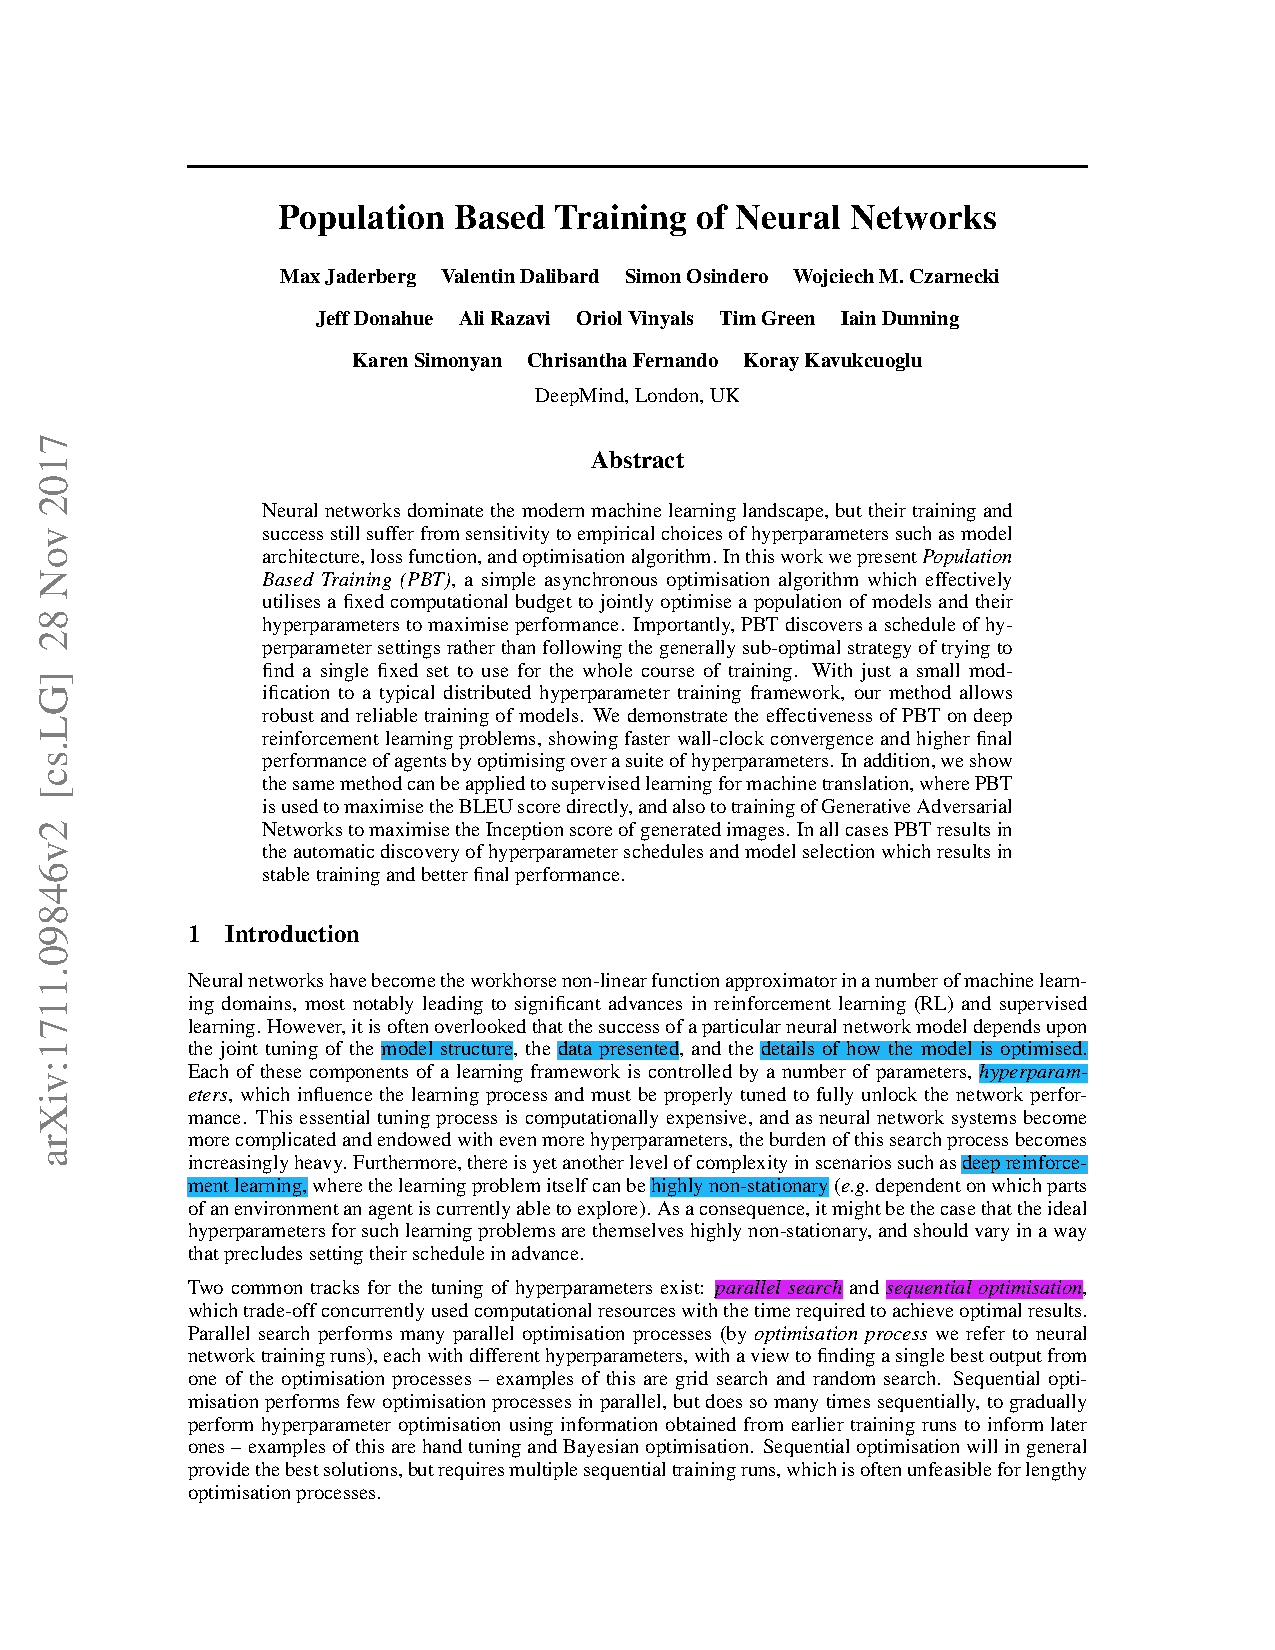
\includepdf[link=true,pages=-,fitpaper]{./papers/Population-Based-Training-of-Neural-Networks.pdf}
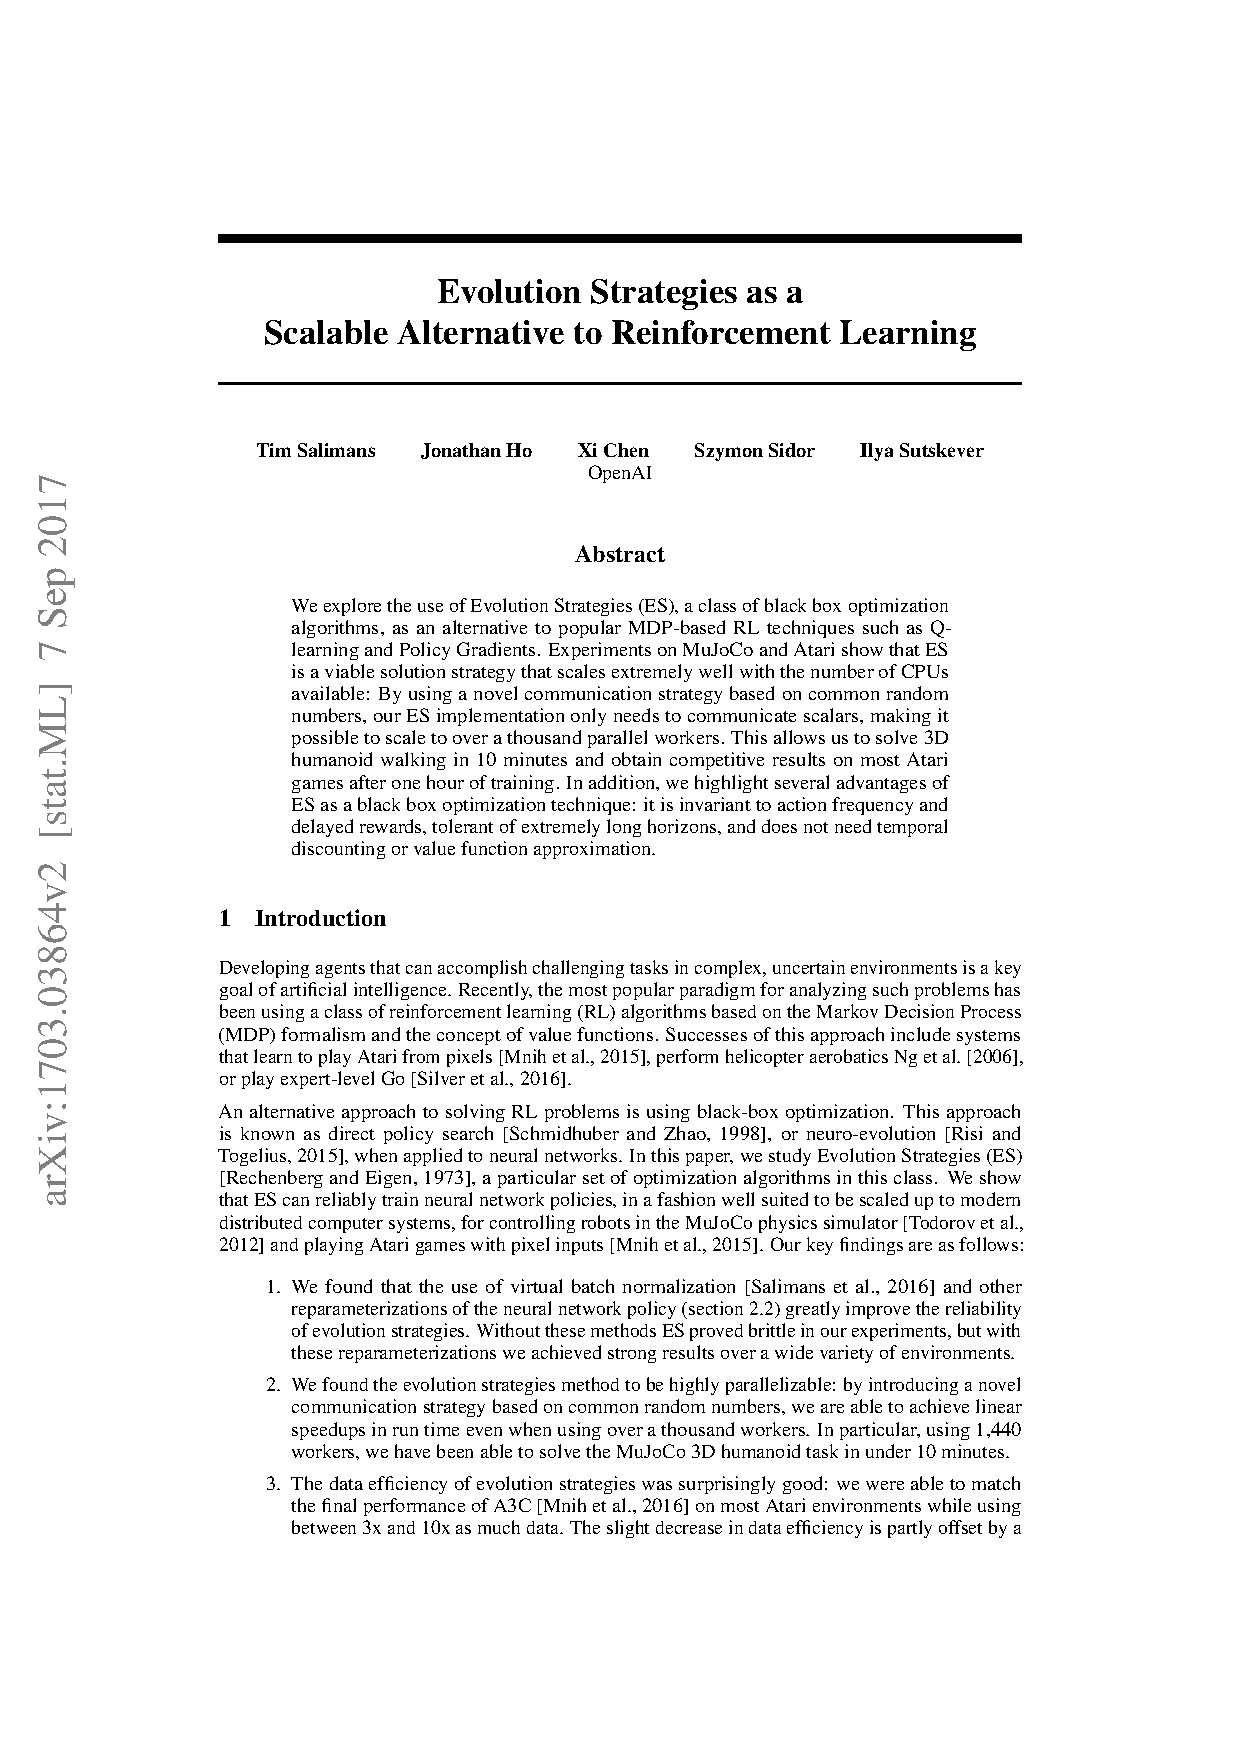
\includepdf[link=true,pages=-,fitpaper]{./papers/Evolution-Strategies-as-a-Scalable-Alternative-to-Reinforcement-Learning.pdf}
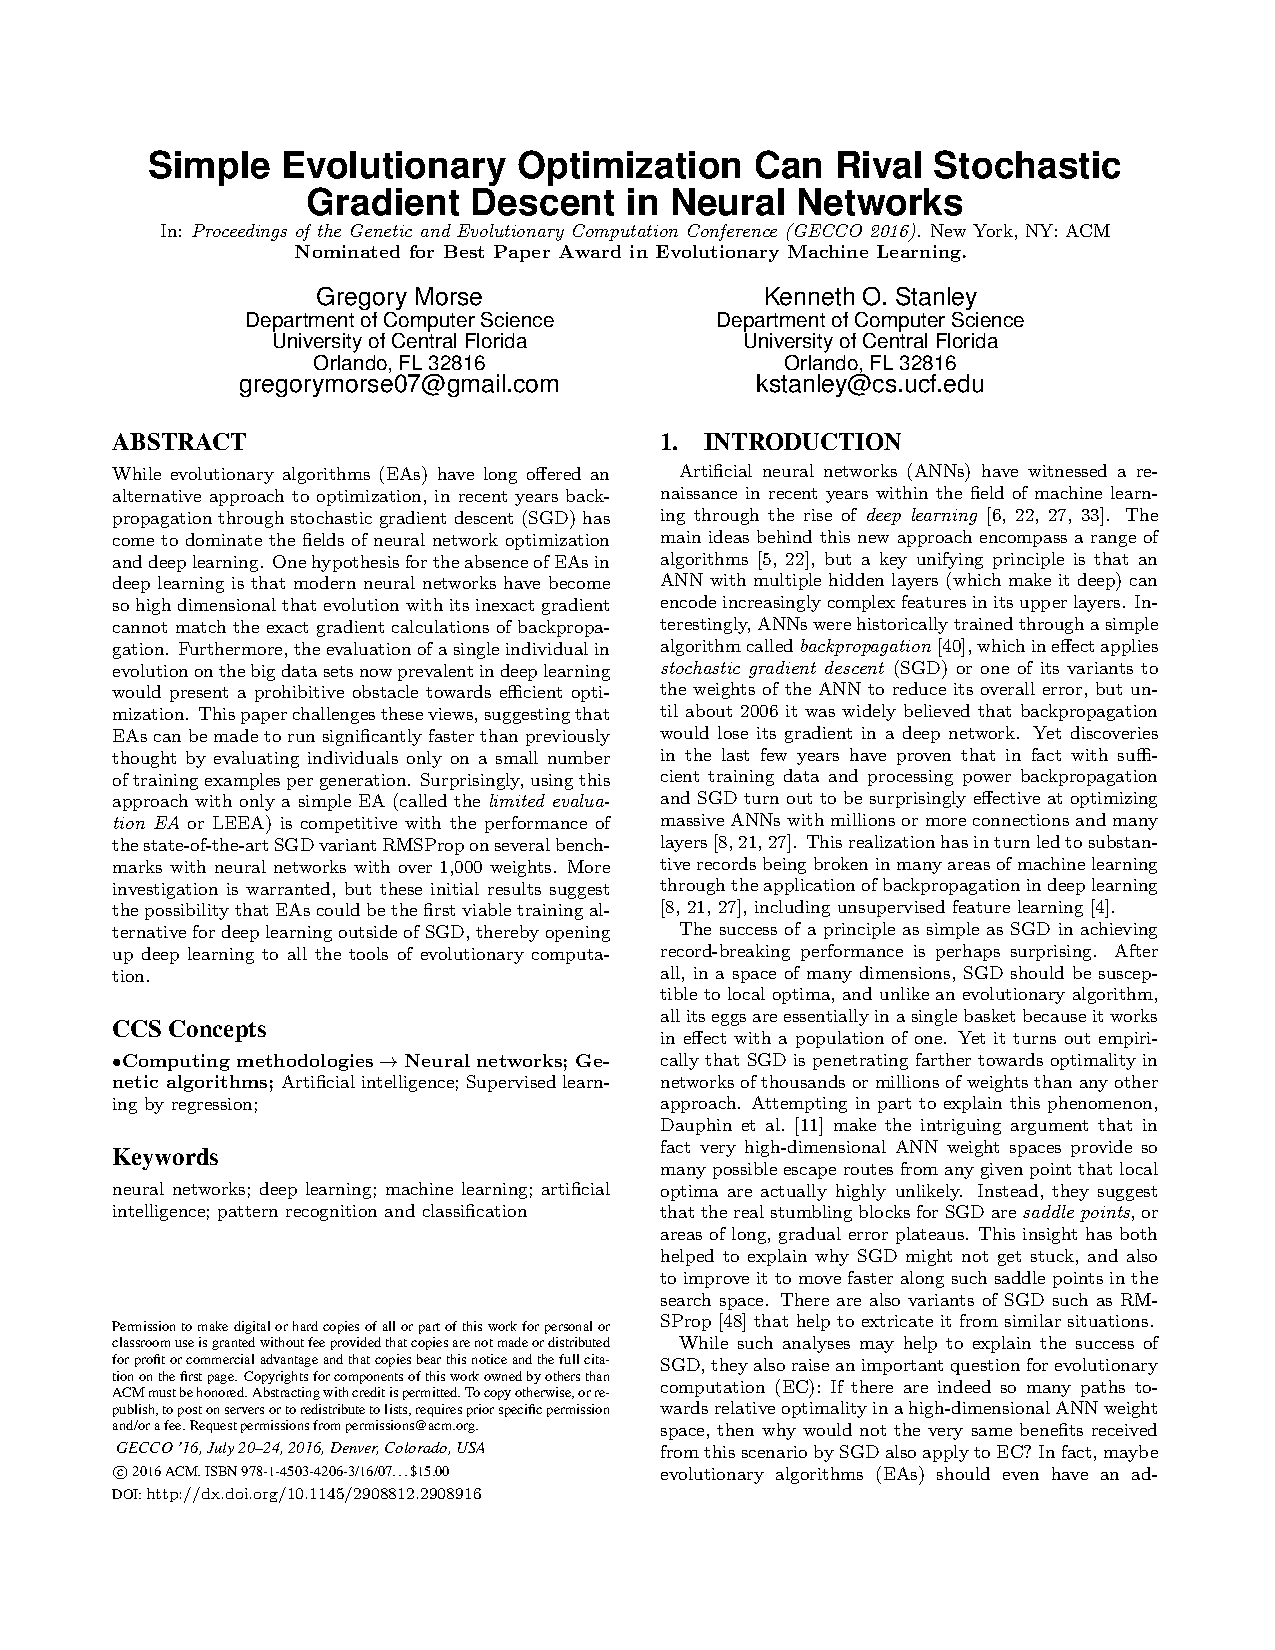
\includepdf[link=true,pages=-,fitpaper]{./papers/Simple-Evolutionary-Optimization-Can-Rival-Stochastic-Gradient-Descent-in-Neural-Networks.pdf}
%\includepdf[link=true,pages=-,fitpaper]{./papers/<++>.pdf}
%\includepdf[link=true,pages=-,fitpaper,angle=-90]{./papers/<++>.pdf}

\end{document}
